\documentclass[11pt,a4paper,twoside,final]{report}
%
\usepackage{ngerman}            %Neue Rechtschreibung
%\usepackage[german]{babel}
\usepackage{graphicx}           %Graphiken einbinden
\usepackage[normalsize]{subfigure}
\usepackage{fontenc}            %Verwenden von \"{o} \"{a} \"{u} {\ss}
\usepackage[utf8]{inputenc}   %Verwenden von \"{o} \"{a} \"{u} {\ss}
\usepackage{fancyhdr}           %Kopf-und Fusszeilen
\usepackage{theorem}
\usepackage{amsmath}
\usepackage{amssymb}
\usepackage{bibgerm}
\usepackage{parskip}
\usepackage{longtable}
\usepackage{helvet}
\usepackage[right]{eurosym}
\usepackage{pdflscape}
\usepackage[compact]{titlesec}
\usepackage{gensymb}
\usepackage[T1]{fontenc}

%\usepackage{pgfplots}
\usepackage{tikz}
\usetikzlibrary{positioning}
\usetikzlibrary{calc}
\usetikzlibrary{shapes.geometric}
\usetikzlibrary{shapes.arrows}
\usetikzlibrary{decorations}
\usetikzlibrary{decorations.pathmorphing}
\usetikzlibrary{decorations.text}
\usetikzlibrary{decorations.markings}
\usetikzlibrary{backgrounds}
\usetikzlibrary{intersections}

\usepackage[a4paper,
			textwidth = 16.5cm,
			textheight = 25cm,
			inner = 2.5cm]{geometry}
		
		
\usepackage[pdftex,
			colorlinks,
			linkcolor = black,
			citecolor = black]{hyperref}
%
%--------------------------------------------------------------------
%
%Kopf- und Fußzeile
%
\pagestyle{fancyplain}
 \renewcommand{\chaptermark}[1]{\markboth{#1}{}}
 \renewcommand{\sectionmark}[1]{\markright{\thesection\ #1}}
 \lhead[\fancyplain{}{\sl\thepage}]{\fancyplain{}{\sl\rightmark}}
 \rhead[\fancyplain{}{\sl\leftmark}]{\fancyplain{}{\sl\thepage}}
 \lfoot{}
 \cfoot{}
 \rfoot{}
%--------------------------------------------------------------------
%
%Definition der Abschnittsüberschriften
%
\titleformat{\chapter}[hang]{\normalfont\large\bfseries}{Aufgabe \thechapter}{6pt}{\large}{}
\renewcommand{\thesection}{\alph{section}}
\titleformat{\section}[runin]{\normalfont}{\thesection )}{6pt}{}
%
%--------------------------------------------------------------------
%
%Kommandos für die Titelseitendaten
%
\newcommand{\VersuchNummer}[1]{\newcommand{\VNummer}{#1}}
\newcommand{\VersuchName}[1]{\newcommand{\VName}{#1}}
\newcommand{\Name}[1]{\newcommand{\SName}{#1}}
\newcommand{\Studiensemester}[1]{\newcommand{\SSemester}{#1}}
\newcommand{\VersuchDatum}[1]{\newcommand{\VDatum}{#1}}
\newcommand{\Mitarbeiter}[1]{\newcommand{\VMitarbeiter}{#1}}
%
%--------------------------------------------------------------------
%
%Titelseite
%
%Daten zum Versuchsprotokoll f�r das Praktikum Elektrische Antriebe
%
%Eingegeben werden:
%
% - Die Nummer und Name des Versuchs:
%     1 Asynchronmaschine
%     2 Gleichstrommaschine
%     3 B�rstenloser Gleichstrommotor
%     4 Schrittmotor
%
\VersuchNummer{1}
\VersuchName{Asynchronmaschine}
%
%------
%
% - Name des Bearbeiters
%
\Name{Max Antriebslos}
%
%------
%
% - Studiensemester des Bearbeiters
\Studiensemester{7}
%
%------
%
% - Datum der Versuchsdurchf�hrung
%
\VersuchDatum{18.10.2014}
%
%------
%
% - Namen der Mitarbeiter in der Gruppe
%
\Mitarbeiter{Johann Ohneland, Hans Lackland}
%
\renewcommand\maketitle{
\begin{titlepage}

\thispagestyle{empty}
%
\begin{tabular}[t]{lp{0.25\textwidth}r}
%

\includegraphics[width = 0.25\textwidth]{./Bilder/Logo_HSRT_TEC_RGB.png}
%
&&
\includegraphics[width = 0.4\textwidth]{./Bilder/Logo_HSRT_Schwarz.jpg}
%
\end{tabular}
%

\renewcommand{\baselinestretch}{1.2}

\sf\large\textbf{Hochschule Reutlingen}\\
\sf\large\textbf{Fakultät Technik}\\

\vspace{7cm}

{\sf\Huge\textbf{Praktikum Elektrische Antriebe}}\\
%
\vspace{0.5cm}

{\sf\huge{Versuchsprotokoll zu  Versuch~\VNummer:}}\\
{\sf\huge{\VName}}

\vspace{4.5cm}

\renewcommand{\arraystretch}{2}
\begin{tabular}{|p{0.33\textwidth}p{0.33\textwidth}p{0.33\textwidth}|}
%
\hline
\multicolumn{2}{|p{0.66\textwidth}|}{Name:~\SName}				&Studiensemester:~\SSemester		\\
\hline
Datum:~\VDatum			      &\multicolumn{2}{|l|}{Testat:}		\\
\hline
\multicolumn{3}{|l|}{Mitarbeiter:~\VMitarbeiter}\\
\hline
%
\end{tabular}
\renewcommand{\arraystretch}{1}

\renewcommand{\baselinestretch}{1}
%

\vfill
%


\includegraphics[width = \textwidth]{./Bilder/Silhouette_HSRT_045K.jpg}
%
\newpage
\ 
\thispagestyle{empty}
%
\end{titlepage}}
%
%--------------------------------------------------------------------
%
\begin{document}
%
\maketitle

\setcounter{page}{1}

%--------------------------------------------------------------------
%
%Mustervorlage fuer eine Aufgabe
%
%--------------------------------------------------------------------
%
%Ueberschreiben der automatisch erzeugten Aufgabennummer
%Die folgende Aufgabennummer ergibt sich aus dem Stand des
%Z�hlers + 1
%\setcounter{chapter}{0}
%
\chapter{}\label{ex:aufg1}
%
%Teilaufgabe 1
%
Siehe Skript Elektrische Antriebe
%

%


%
%Alle bisherigen Bilder einf�gen und einen Seitenumbruch erzwingen
\clearpage

%--------------------------------------------------------------------
%
%Mustervorlage fuer eine Aufgabe
%
%--------------------------------------------------------------------
%
%Ueberschreiben der automatisch erzeugten Aufgabennummer
%Die folgende Aufgabennummer ergibt sich aus dem Stand des
%Zählers + 1
%\setcounter{chapter}{0}
%
\chapter{}\label{ex:aufg2}
%
%Teilaufgabe 1
%
\section{}\label{sec:aufg2a}
%
In den folgenden Graphiken (siehe Abb. \ref{dia:aufg2a_hall})sehen Sie die Signale der Hallsensoren(siehe Abb. \ref{dia:aufg2a_hall}) und die idealisierten Stromverläufe(siehe Abb. \ref{dia:aufgabe2a_strom}).
\begin{figure}[htb]
	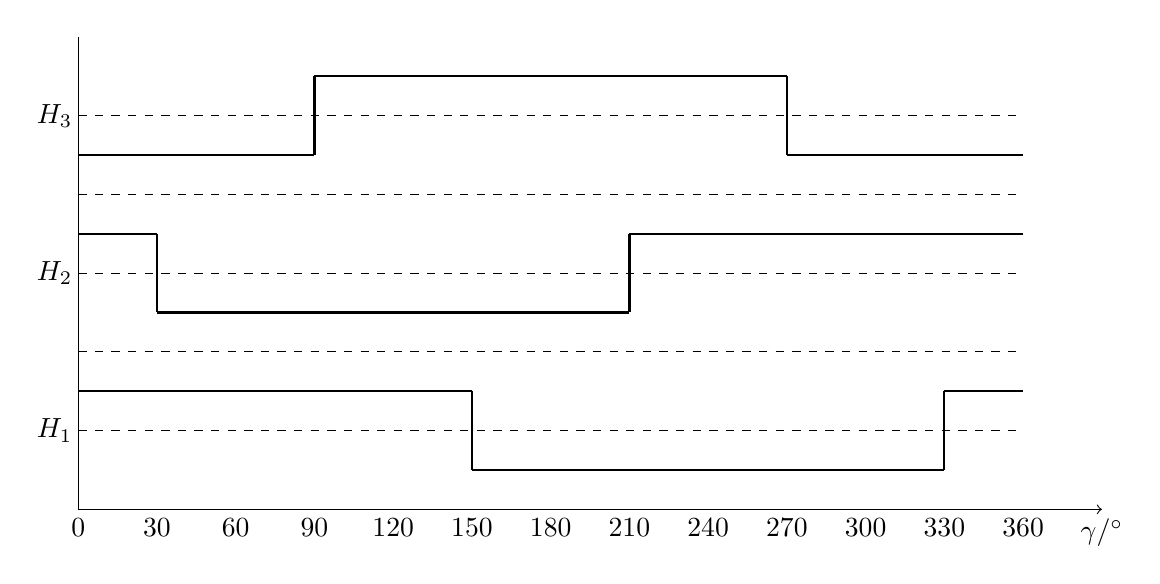
\begin{tikzpicture}
	
	% horizontal axis
	\draw[->] (0,0) -- (13,0) node[anchor=north] {$\gamma/^{\circ}$};
	\draw[dashed] (0, 1) -- (12,1);
	\draw[dashed] (0, 2) -- (12,2);
	\draw[dashed] (0, 3) -- (12,3);
	\draw[dashed] (0, 4) -- (12,4);
	\draw[dashed] (0, 5) -- (12,5);

	% vertical axis
	\draw (0,0) -- (0,6) node[anchor=east] {};

	% labels
	\draw	(0,0) node[anchor=north] {0}
	(1,0) node[anchor=north] {30}
	(2,0) node[anchor=north] {60}
	(3,0) node[anchor=north] {90}	
	(4,0) node[anchor=north] {120}
	(5,0) node[anchor=north] {150}
	(6,0) node[anchor=north] {180}
	(7,0) node[anchor=north] {210}
	(8,0) node[anchor=north] {240}
	(9,0) node[anchor=north] {270}
	(10,0) node[anchor=north] {300}
	(11,0) node[anchor=north] {330}
	(12,0) node[anchor=north] {360};	
	
	\draw (-0.3, 5) node{{$H_3$}};
	\draw (-0.3, 3) node{{$H_2$}};
	\draw (-0.3, 1) node{{$H_1$}};

	%draw H3
	\draw [thick] (0, 4.5) -- (3, 4.5)
	(3, 4.5) -- (3, 5.5)
	(3, 5.5) -- (9, 5.5)
	(9, 5.5) -- (9, 4.5)
	(9, 4.5) -- (12, 4.5);
	
	%draw H2
	\draw [thick] (0, 3.5) -- (1, 3.5)
	(1, 3.5) -- (1, 2.5)
	(1, 2.5) -- (7, 2.5)
	(7, 2.5) -- (7, 3.5)
	(7, 3.5) -- (12, 3.5);
	
	%draw H1
	\draw [thick] (0, 1.5) -- (5, 1.5)
	(5, 1.5) -- (5, 0.5)
	(5, 0.5) -- (11, 0.5)
	(11, 0.5) -- (11, 1.5)
	(11, 1.5) -- (12, 1.5);


	
	\end{tikzpicture}
	\caption{Signale der Hallsensoren - Rechtslauf}
	\label{dia:aufg2a_hall}
\end{figure}

\begin{figure}[htb]
	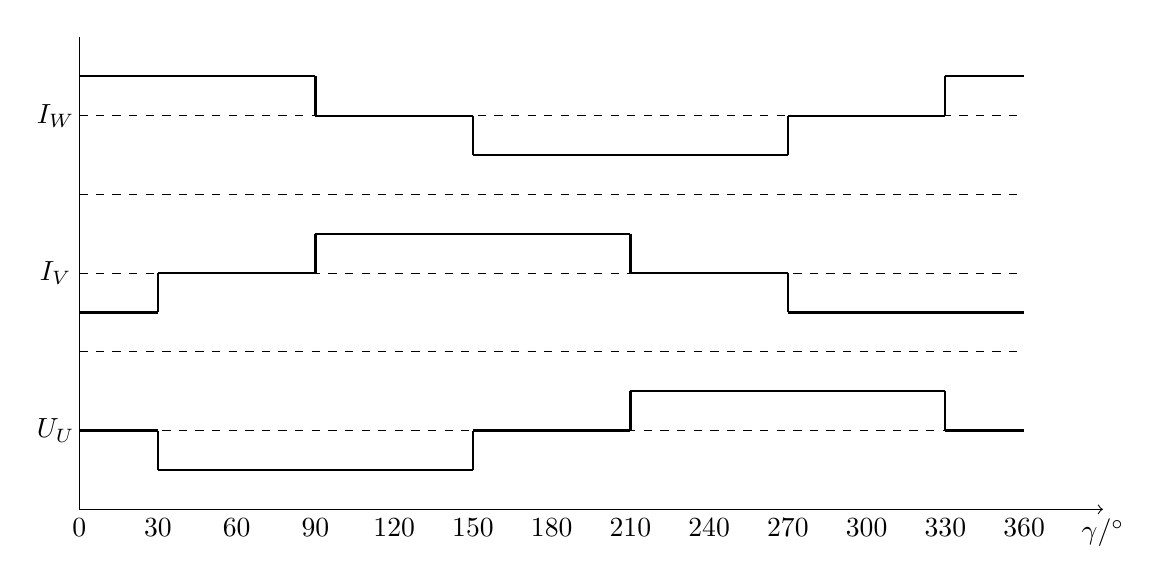
\begin{tikzpicture}
	
	% horizontal axis
	\draw[->] (0,0) -- (13,0) node[anchor=north] {$\gamma/^{\circ}$};
	\draw[dashed] (0, 1) -- (12,1);
	\draw[dashed] (0, 2) -- (12,2);
	\draw[dashed] (0, 3) -- (12,3);
	\draw[dashed] (0, 4) -- (12,4);
	\draw[dashed] (0, 5) -- (12,5);
	
	% vertical axis
	\draw (0,0) -- (0,6) node[anchor=east] {};
	
	% labels
	\draw	(0,0) node[anchor=north] {0}
	(1,0) node[anchor=north] {30}
	(2,0) node[anchor=north] {60}
	(3,0) node[anchor=north] {90}	
	(4,0) node[anchor=north] {120}
	(5,0) node[anchor=north] {150}
	(6,0) node[anchor=north] {180}
	(7,0) node[anchor=north] {210}
	(8,0) node[anchor=north] {240}
	(9,0) node[anchor=north] {270}
	(10,0) node[anchor=north] {300}
	(11,0) node[anchor=north] {330}
	(12,0) node[anchor=north] {360};	
	
	\draw (-0.3, 5) node{{$I_W$}};
	\draw (-0.3, 3) node{{$I_V$}};
	\draw (-0.3, 1) node{{$U_U$}};
	
	%draw Iw
	\draw [thick] 
	(0, 5.5)  --  (3, 5.5)
	(3, 5.5)  --  (3, 5.0)
	(3, 5.0)  --  (5, 5.0)
	(5, 5.0)  --  (5, 4.5)
	(5, 4.5)  --  (9, 4.5)
	(9, 4.5)  --  (9, 5.0)
	(9, 5.0)  -- (11, 5.0)
	(11, 5.0) -- (11, 5.5)
	(11, 5.5) -- (12, 5.5);
	
	%draw Iv
	\draw [thick] 
	(0, 2.5)  --  (1, 2.5)
	(1, 2.5)  --  (1, 3.0)
	(1, 3.0)  --  (3, 3.0)
	(3, 3.0)  --  (3, 3.5)
	(3, 3.5)  --  (7, 3.5)
	(7, 3.5)  --  (7, 3.0)
	(7, 3.0)  --  (9, 3.0)
	(9, 3.0)  --  (9, 2.5)
	(9, 2.5)  -- (12, 2.5);
	
	%draw Iu
	\draw [thick] 
	(0, 1.0)  --  (1, 1.0)
	(1, 1.0)  --  (1, 0.5)
	(1, 0.5)  --  (5, 0.5)
	(5, 0.5)  --  (5, 1.0)
	(5, 1.0)  --  (7, 1.0)
	(7, 1.0)  --  (7, 1.5)
	(7, 1.5)  -- (11, 1.5)
	(11, 1.5) -- (11, 1.0)
	(11, 1.0) -- (12, 1.0);
	
	\end{tikzpicture}
	\caption{Idealisierte Stromverl\"aufe}
	\label{dia:aufgabe2a_strom}
\end{figure}
\newpage
%
%--------------------------------------------------------------------
%
%Teilaufgabe 2
%
\section{}\label{sec:aufg2b}
%
In dem folgenden Diagramm (siehe Abb.\ref{dia:2b_ansteuersig}) werden die Ansteuersignale der sechs Transistoren für den Rechtslauf dargestellt. Der Einfachheit halber werden für $W$,$V$ und $U$ je Highside leitend als $1$, Lowside leitend als $-1$ und gesperrt als $0$ bezeichnet. Somit gleichen die Ansteuersignale dem idealisierten Stromverlauf aus dem Skript elektische Antriebe S.102, Abb. 8.3.
\begin{figure}[htb]
	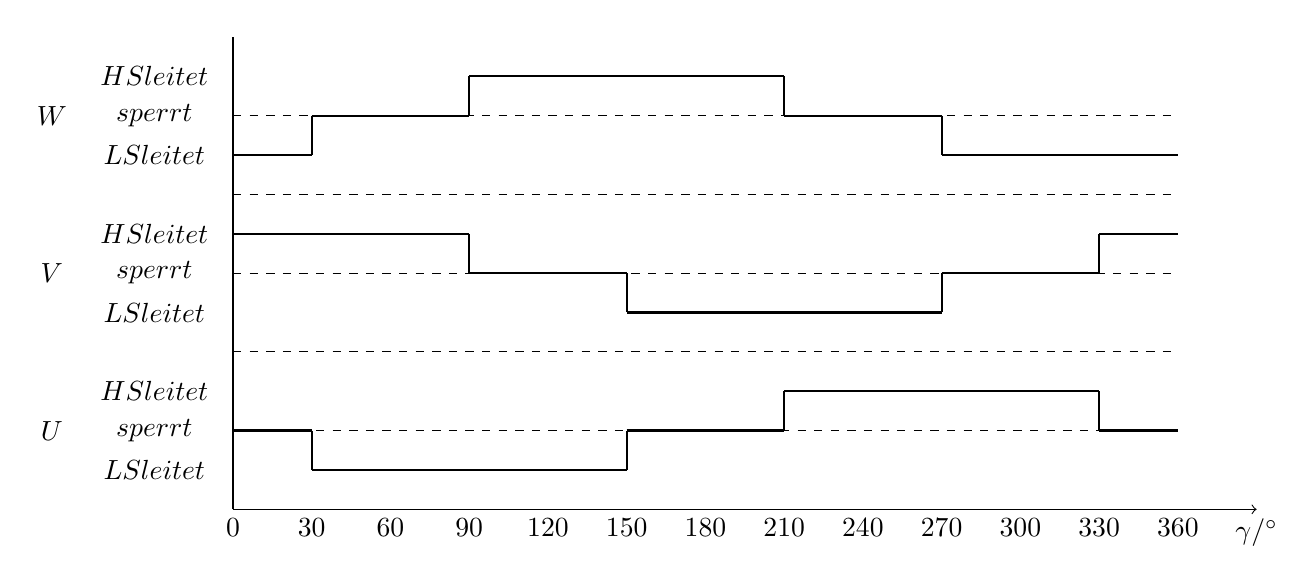
\begin{tikzpicture}
	
		% horizontal axis
		\draw[->] (0,0) -- (13,0) node[anchor=north] {$\gamma/^{\circ}$};
		\draw[dashed] (0, 1) -- (12,1);
		\draw[dashed] (0, 2) -- (12,2);
		\draw[dashed] (0, 3) -- (12,3);
		\draw[dashed] (0, 4) -- (12,4);
		\draw[dashed] (0, 5) -- (12,5);
		
		% vertical axis
		\draw (0,0) -- (0,6) node[anchor=east] {};
		
		% labels
		\draw	(0,0) node[anchor=north] {0}
		(1,0) node[anchor=north] {30}
		(2,0) node[anchor=north] {60}
		(3,0) node[anchor=north] {90}	
		(4,0) node[anchor=north] {120}
		(5,0) node[anchor=north] {150}
		(6,0) node[anchor=north] {180}
		(7,0) node[anchor=north] {210}
		(8,0) node[anchor=north] {240}
		(9,0) node[anchor=north] {270}
		(10,0) node[anchor=north] {300}
		(11,0) node[anchor=north] {330}
		(12,0) node[anchor=north] {360};	
		
		\draw (-2.3, 5) node{{$W$}};
			\draw (-1, 5.5) node{{$HS leitet$}};
			\draw (-1, 5) node{{$sperrt$}};
			\draw (-1, 4.5) node{{$LS leitet$}};
		\draw (-2.3, 3) node{{$V$}};
			\draw (-1, 3.5) node{{$HS leitet$}};
			\draw (-1, 3) node{{$sperrt$}};
			\draw (-1, 2.5) node{{$LS leitet$}};
		\draw (-2.3, 1) node{{$U$}};
			\draw (-1, 1.5) node{{$HS leitet$}};
			\draw (-1, 1) node{{$sperrt$}};
			\draw (-1, 0.5) node{{$LS leitet$}};
		
		%draw W
		\draw [thick] 
		(0, 4.5)  --  (1, 4.5)
		(1, 4.5)  --  (1, 5.0)
	 	(1, 5.0)  --  (3, 5.0)
		(3, 5.0)  --  (3, 5.5)
		(3, 5.5)  --  (7, 5.5)
		(7, 5.5)  --  (7, 5.0)
		(7, 5.0)  --  (9, 5.0)
		(9, 5.0)  --  (9, 4.5)
		(9, 4.5)  -- (12, 4.5);
		
		%draw V
		\draw [thick] 
		(0, 3.5)  --  (3, 3.5)
		(3, 3.5)  --  (3, 3.0)
		(3, 3.0)  --  (5, 3.0)
		(5, 3.0)  --  (5, 2.5)
		(5, 2.5)  --  (9, 2.5)
		(9, 2.5)  --  (9, 3.0)
		(9, 3.0)  -- (11, 3.0)
		(11, 3.0) -- (11, 3.5)
		(11, 3.5) -- (12, 3.5);
		
		%draw U
		\draw [thick] 
		(0, 1.0)  --  (1, 1.0)
		(1, 1.0)  --  (1, 0.5)
		(1, 0.5)  --  (5, 0.5)
		(5, 0.5)  --  (5, 1.0)
		(5, 1.0)  --  (7, 1.0)
		(7, 1.0)  --  (7, 1.5)
		(7, 1.5)  -- (11, 1.5)
		(11, 1.5) -- (11, 1.0)
		(11, 1.0) -- (12, 1.0);
	
	\end{tikzpicture}
	\caption{Ansteuersignale der 6 Transistoren - Rechtslauf}
	\label{dia:2b_ansteuersig}
\end{figure}
%
\section{}\label{sec:aufg2c}
%
Die Ansteuerung der Transistoren entspricht wir in (\ref{sec:aufg2b}) erwähnt  dem idealisierten Stromverlauf.
\begin{figure}[htb]
	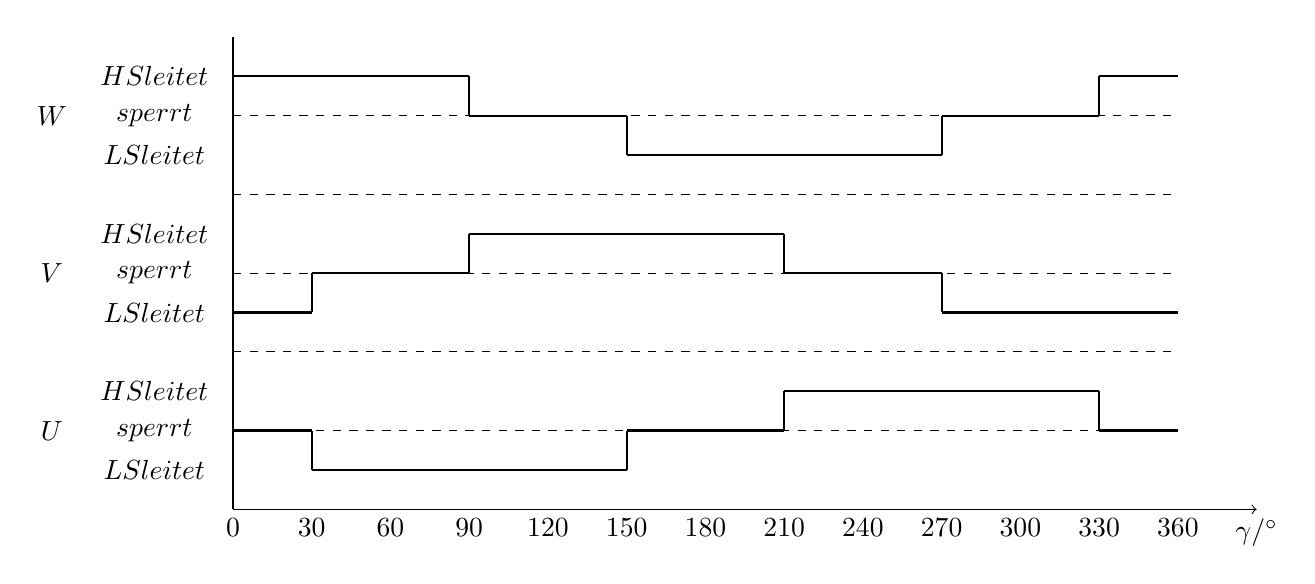
\begin{tikzpicture}
	
		% horizontal axis
		\draw[->] (0,0) -- (13,0) node[anchor=north] {$\gamma/^{\circ}$};
		\draw[dashed] (0, 1) -- (12,1);
		\draw[dashed] (0, 2) -- (12,2);
		\draw[dashed] (0, 3) -- (12,3);
		\draw[dashed] (0, 4) -- (12,4);
		\draw[dashed] (0, 5) -- (12,5);
		
		% vertical axis
		\draw (0,0) -- (0,6) node[anchor=east] {};
		
		% labels
		\draw	(0,0) node[anchor=north] {0}
		(1,0) node[anchor=north] {30}
		(2,0) node[anchor=north] {60}
		(3,0) node[anchor=north] {90}	
		(4,0) node[anchor=north] {120}
		(5,0) node[anchor=north] {150}
		(6,0) node[anchor=north] {180}
		(7,0) node[anchor=north] {210}
		(8,0) node[anchor=north] {240}
		(9,0) node[anchor=north] {270}
		(10,0) node[anchor=north] {300}
		(11,0) node[anchor=north] {330}
		(12,0) node[anchor=north] {360};	
		
		\draw (-2.3, 5) node{{$W$}};
			\draw (-1, 5.5) node{{$HS leitet$}};
			\draw (-1, 5) node{{$sperrt$}};
			\draw (-1, 4.5) node{{$LS leitet$}};
		\draw (-2.3, 3) node{{$V$}};
			\draw (-1, 3.5) node{{$HS leitet$}};
			\draw (-1, 3) node{{$sperrt$}};
			\draw (-1, 2.5) node{{$LS leitet$}};
		\draw (-2.3, 1) node{{$U$}};
			\draw (-1, 1.5) node{{$HS leitet$}};
			\draw (-1, 1) node{{$sperrt$}};
			\draw (-1, 0.5) node{{$LS leitet$}};
		
		%draw W
		\draw [thick] 
		(0, 5.5)  --  (3, 5.5)
		(3, 5.5)  --  (3, 5.0)
		(3, 5.0)  --  (5, 5.0)
		(5, 5.0)  --  (5, 4.5)
		(5, 4.5)  --  (9, 4.5)
		(9, 4.5)  --  (9, 5.0)
		(9, 5.0)  -- (11, 5.0)
		(11, 5.0) -- (11, 5.5)
		(11, 5.5) -- (12, 5.5);
		
		%draw V
		\draw [thick] 
		(0, 2.5)  --  (1, 2.5)
		(1, 2.5)  --  (1, 3.0)
		(1, 3.0)  --  (3, 3.0)
		(3, 3.0)  --  (3, 3.5)
		(3, 3.5)  --  (7, 3.5)
		(7, 3.5)  --  (7, 3.0)
		(7, 3.0)  --  (9, 3.0)
		(9, 3.0)  --  (9, 2.5)
		(9, 2.5)  -- (12, 2.5);
		
		%draw U
		\draw [thick] 
		(0, 1.0)  --  (1, 1.0)
		(1, 1.0)  --  (1, 0.5)
		(1, 0.5)  --  (5, 0.5)
		(5, 0.5)  --  (5, 1.0)
		(5, 1.0)  --  (7, 1.0)
		(7, 1.0)  --  (7, 1.5)
		(7, 1.5)  -- (11, 1.5)
		(11, 1.5) -- (11, 1.0)
		(11, 1.0) -- (12, 1.0);
	
	\end{tikzpicture}
	\caption{Ansteuersignale der 6 Transistoren - Linkslauf}
	\label{dia:2c_ansteuersig}
\end{figure}
%
\newpage
\section{}\label{sec:aufg2d}
%
Wir nutzen die Formel 5.9 aus dem Vorlesungsskript S.41.
\begin{equation}
	U_a = R_a I_a(t) + L_a \frac{dI_a(t)}{dt} + U_I
	\label{for:formel1}
\end{equation}

Da $U_I = 0$ kommen wir zu folgender Formel:
\begin{equation}
	I_a(t) = \frac{U_a - L_a \frac{dI_a(t)}{dt}}{R_a}
	\label{for:formel2}
\end{equation}

Umgeformt ergibt das:
\begin{equation}
	\tau\frac{dI_a(t)}{dt} + I_a(t) = \frac{U_a}{R_a}
\end{equation}

Die Lösung der Differentialgleichung ergibt:
\begin{equation}
	I_a(t) = \frac{U_a}{R_a}(1-e^-\frac{t-1ms}{\tau})
\end{equation}
Für $R_a = 0.8 \Omega$ und $L_a = 1.1 mH$ und einem Spannungsverlauf, wie im Srkipt (siehe S.105 Abb. 8.7) dargestellt, ergibt es im Strang U einen Ankerstrom der folgendermaßen verläuft(siehe Abb.\ref{fig:ankerstrom}):
\begin{figure}[htb]
	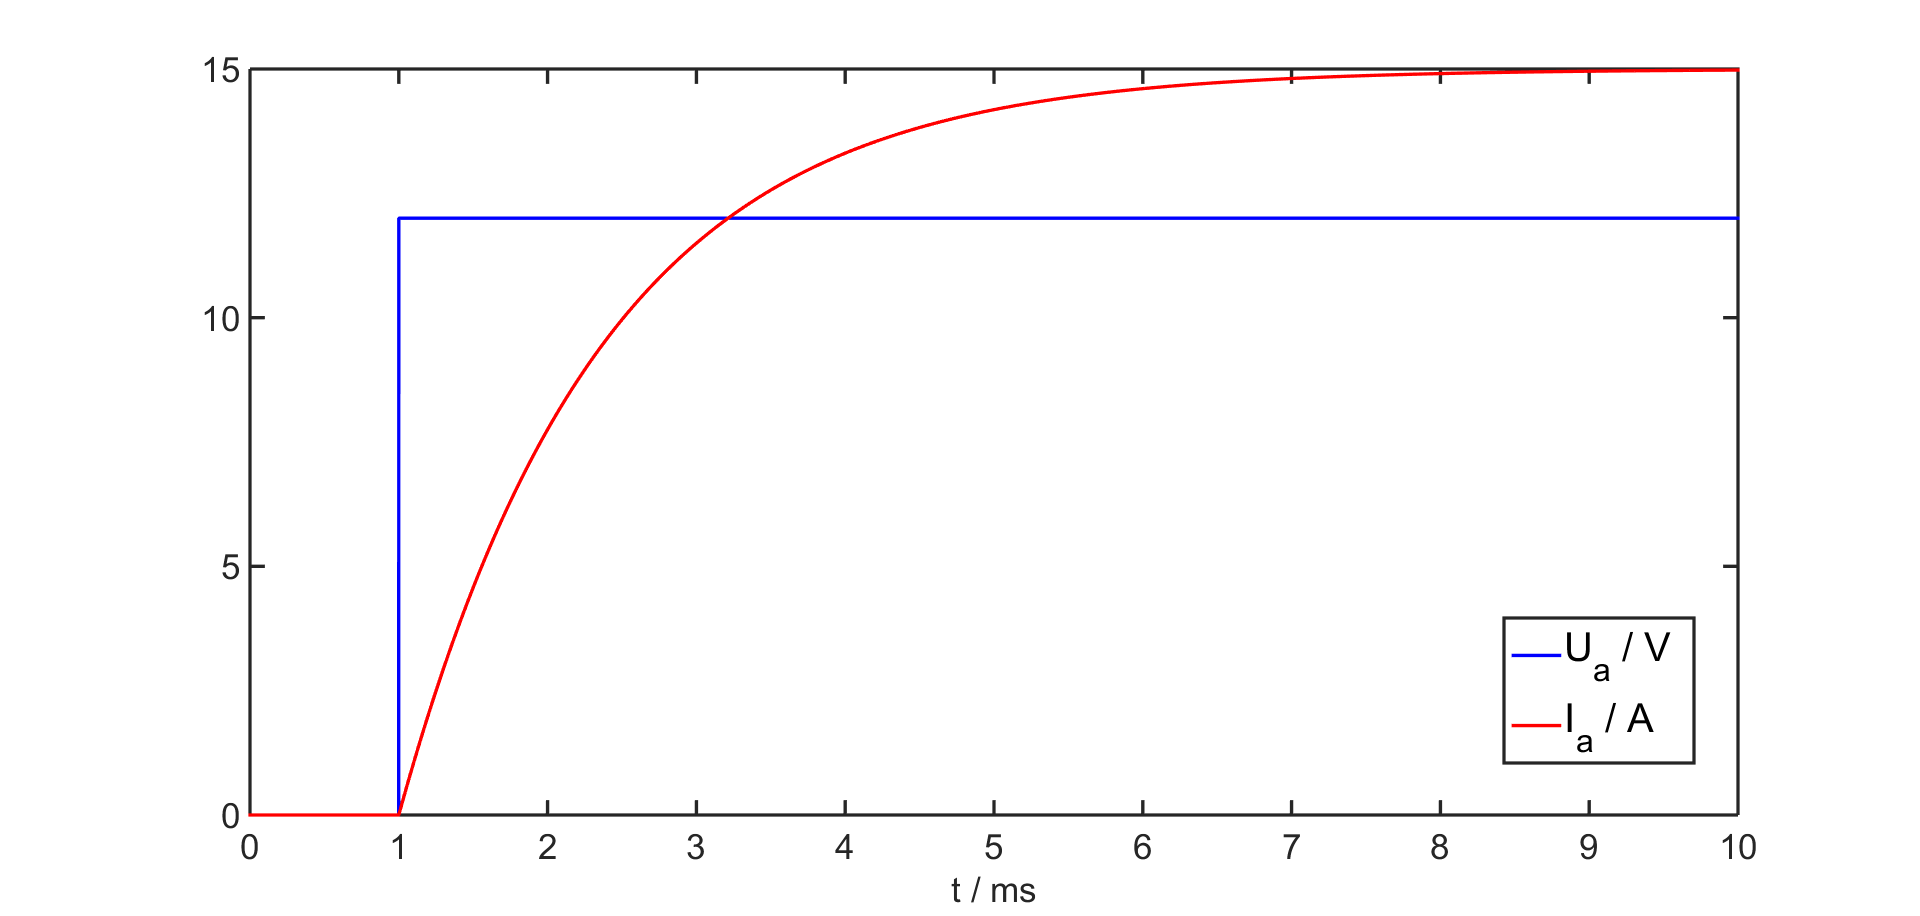
\includegraphics[width=\textwidth]{./Bilder/Ankerstrom_Aufgabe2d}
	\caption{Verlauf des Ankerstroms}
	\label{fig:ankerstrom}
\end{figure}




%\begin{tikzpicture}

\begin{axis}[xmax = 10, ymax = 15, samples=100]
\addplot[blue, ultra thick] (x,x*x)
\end{axis}

\end{tikzpicture}

%Alle bisherigen Bilder einfügen und einen Seitenumbruch erzwingen
\clearpage

\chapter{}\label{ex:aufg3}
%
\section{}\label{sec:aufg3a}
Mit Gleichung (5.12) aus dem Skript elektrische Antriebe kann $c_\text{E} \Psi_\text{N}$ berechnet werden. Dazu wird die Gleichstrommaschine im generatorischen Betrieb verwendet, das bedeutet, die Synchronmaschine bestimmt die Drehzahl, die Gleichstrommaschine liefert kein Drehmoment.Im Leerlauf gilt somit $M_{Mi} = 0$, daraus folgt
\begin{equation}
c_\text{E} \Psi_\text{N} = \frac{U_{\text{AN}}}{N_{\text{N}0}}
\end{equation} 
Mit Gleichung (5.6) und (5.11) aus dem Skript elektrische Antriebe erhält man
\begin{equation}
R_A = \frac{U_{\text{AN}} - c_\text{E} \Psi_\text{N} \cdot N_\text{N}}{I_{\text{AN}}}
\end{equation} 

\section{}\label{sec:aufg3b}
%
%$U_A = 179.2\text{V}, N_{N0} = 1792min^-1$
Für $c_\text{E} \Psi_\text{N}$ ergab sich $c_E \Psi_N = 6.016 \text{Vs}$.
Die Berechnung von $R_\text{A}$ wurde erst mit den Werten des Typenschilds durchgeführt.
\begin{equation}
R_\text{A} = \frac{U_{\text{AN}} - c_\text{E} \Psi_\text{N} \cdot N_\text{N}}{I_{\text{AN}}} = \frac{210 \text{V} - 6.016\text{Vs} \cdot \frac{1900}{60\text{s}}}{1.61\text{A}} = 12.1078 \Omega
\end{equation}
Nach der Messung der Werte U, I und N ergab sich für $R_\text{A} = 8.12\Omega$.
%$U_A = 100 \text{V}, I_A = 0 \text{A}, N_0 = 1040 \frac{1}{\text{min}}, I_{AN} = 1.61\text{A}$

\clearpage
\chapter{}\label{ex:aufg4}
%
\section{}\label{sec:aufg4a}
Mit den Gleichungen (5.6) und (5.11) aus dem Skript Elektrische Antriebe ergibt sich für $c_\text{E}\Psi(I_\text{E})$
\begin{equation}
c_\text{E}\Psi(I_\text{E}) = \frac{U_\text{A} - R_\text{A} \cdot I_\text{A}}{N(I_\text{E})}
\end{equation}
\section{}\label{sec:aufg4b}
Wenn der Erregerstrom $I_E$ unabhängig zur Ankerspannung abgeschaltet wird, ist die Flussverkettung niedrig, das führt zu einer sehr hohen Leerlaufdrehzahl, welche den Motor mechanisch zerstören kann. Eine Möglichkeit wäre nun, den Erregerstrom nicht bis auf null zu fahren, allerdings erhält man dann nicht die komplette Magnetisierungskennlinie.

Sinnvoller ist es, den Motor analog zu Aufgabe 3a im generatorischen Betrieb zu verwenden. Somit ist $I_A$ null, durch die Messung der induzierten Ankerspannung und der Drehzahl lässt sich $c_\text{E}\Psi(I_\text{E})$ berechnen.

\section{}\label{sec:aufg4c}
%
In Abb. \ref{fig:magnet} ist die gemessene Magnetisierungskennlinie dargestellt.
\begin{figure}[htb]

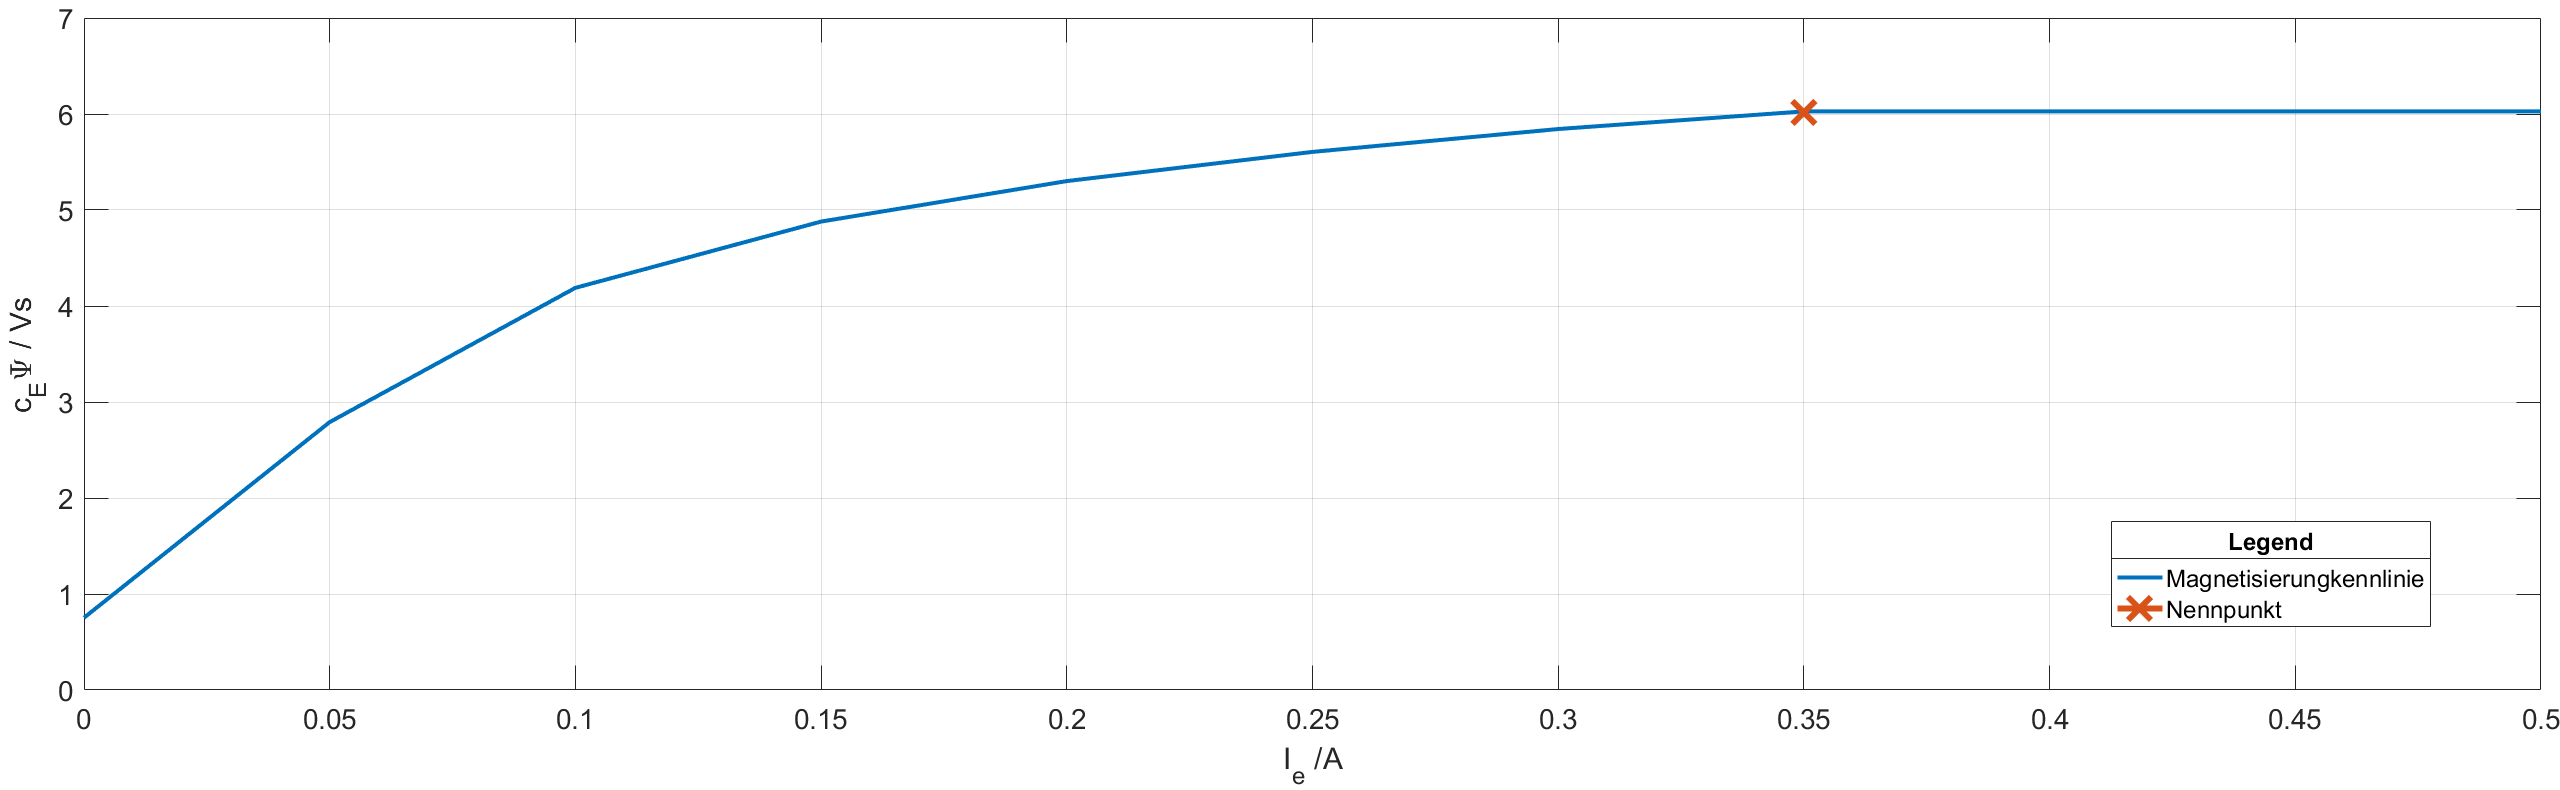
\includegraphics[width=1\textwidth]{./Bilder/magentisierungkennlinie_1}
\caption{Magnetisierungskennlinie}
\label{fig:magnet}
\end{figure}
%
\section{}\label{sec:aufg4_d}
%
Der Erregerstrom wird so eingestellt, dass eine Nennflussverkettung $\Psi_\text{N} = 6.016$Vs erreicht wird. Bei einem höheren Erregerstrom würde die Nennflussverkettung nicht, bzw. kaum steigen, weil der Eisenkern sich in Sättigung befindet. Bei niedrigeren Erregerströmen tritt bei schwankender Spannungsversorgung eine große Änderung des Flusses auf, da die Steigung der Magnetisierungskennlinie(siehe Abb. \ref{fig:magnet}) in diesem Bereich sehr hoch ist. Außerdem wird bei einer Absenkung des Feldes das Nennmoment erreicht (Feldschwächbereich).
%
\clearpage
\chapter{}\label{ex:aufg5}
%
\section{}\label{sec:aufg5a}
%
In Abb. \ref{fig:drehzahldrehm} werden die Drehzahlen des BLDCs bei den Ankerspannungen $U_A = 20V$, $U_A = 15V$ und $U_A = 10V$ in Abhängigkeit des Lastdrehmoments dargestellt.

\begin{figure}[htb]
	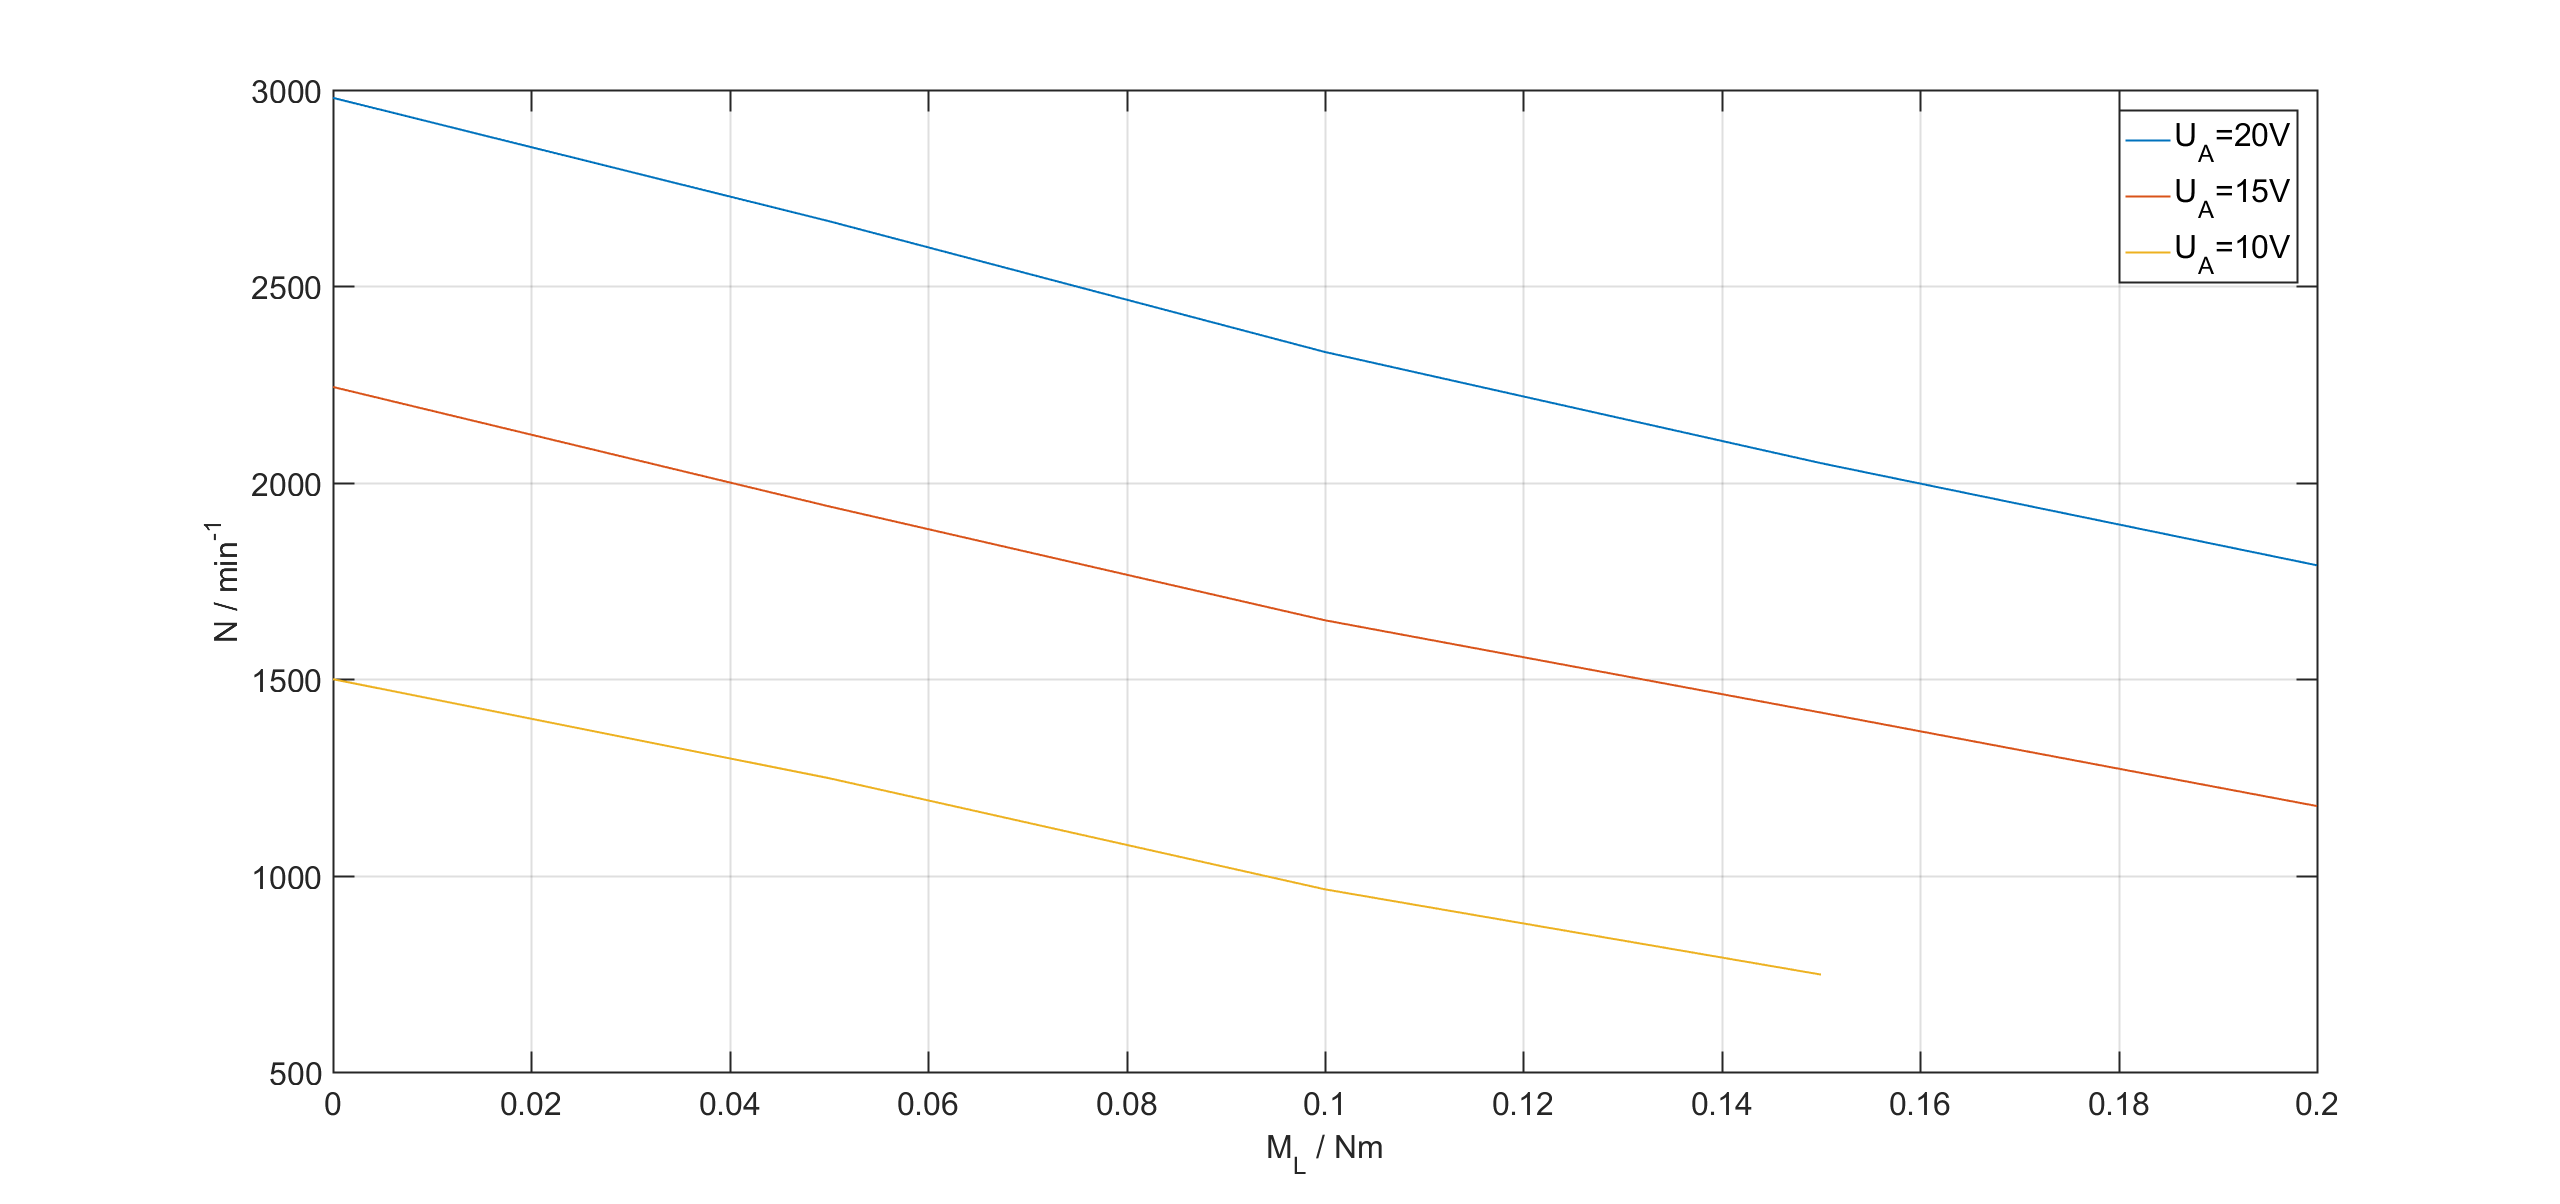
\includegraphics[width = \textwidth]{./Bilder/Drehzahldrehmomentkennlinie}
	\caption{Drehzahl-Drehmomentkennline}
	\label{fig:drehzahldrehm}
\end{figure}
%
\section{}\label{sec:aufg5b}
%
In Abb. \ref{fig:drehzahldrehm} erkennt man, dass es bei einer Ankerspannung von $10V$ nicht möglich ist, ein Drehmoment von $0.2 Nm$ zu erreichen. Dies rührt daher, dass der BLDC einen DC-Motor antreibt, welcher generatorisch wirkt und somit eine Spannung erzeugt. Diese verursacht einen Stromfluss durch einen veränderlichen ohmschen Widerstand, dessen Größe durch den Laststrom-Regler angepasst werden kann. Bei $10V$ hat der BLDC eine bestimmte Drehzahl, somit kann nur eine bestimmte Spannung am Generator erzeugt werden. Der größtmögliche Strom am DC-Motor und damit auch das maximal erreichbare Lastmoment wird nach dem ohmschen Gesetz durch die Größe des Widerstands begrenzt. Selbst wenn dieser den kleinsten möglichen Wert annimmt, wird lediglich ein Strom von ca. $3A$ und das entsprechende Drehmoment von ungefähr $0,15Nm$ erzeugt.
\chapter{}\label{ex:aufg6}
%
\section{}\label{sec:aufg6a}
%
Da die Kennlinie aus Abb. \ref{dia:uf_kennlinie} sich auf den Scheitelwert der Statorspannung bezieht, wir aber den Effektivwert der Außenleiterspannung
 benötigen muss dieser noch durch $\sqrt 2$ geteilt und mit $\sqrt 3$ mutlipliziert werden.
Als Faktor wird die Streigung der Kennlinie verwendet
\begin{equation}
	U_{\text{max}} = \frac{317~\text{V}}{\sqrt{2}} \cdot \sqrt{3} = 388 \text{V}
\end{equation}
\begin{equation}
	m = \frac{U_{\text{max}}}{f_{\text{Knick}}} = \frac{388~\text{V}}{50~\text{Hz}}
\end{equation}
%
\section{}\label{sec:aufg6b}
%

%
\section{}\label{sec:aufg6c}
%

%
%und möglicherweise noch andere Aufgaben
%

%
\end{document}

